% XeLaTeX
\documentclass[zh]{report}

\title {My \LaTeX\ Template}
\author{pastglory\thanks{\href{mailto:sunyata000@hotmail.com}{sunyata000@hotmail.com}}}

\begin{document}
\maketitle

Hello, \LaTeX.
This is a paper\cite{zhang2020sparch}.
% 你好,\LaTeX!这是另一篇论文\cite{sadi2017design}. 现在使用一句长句来调行间距,以达到
% 自定义命令的需求

% 下图为FPGA基本单元结构图。
\begin{figure}[H] % H为当前位置,!htb为忽略美学标准,htbp为浮动图形
    \centering
    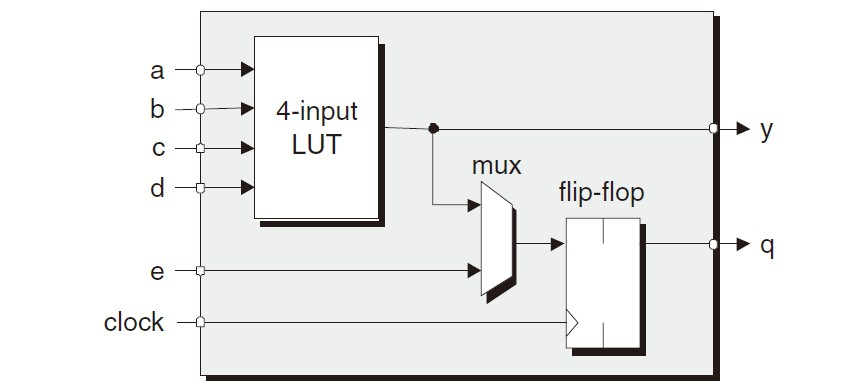
\includegraphics{img/FPGA.jpg}
    \caption{Slice of FPGA} %最终文档中希望显示的图片标题
    \label{图1} %用于文内引用的标签
\end{figure}

\bibliography{reference}

\end{document}
